\documentclass[../main.tex]{subfiles}
\graphicspath{{\subfix{../img/}}}

\begin{document}

% \thispagestyle{empty}
% \etocignoretoctocdepth % of course, if we want to see something in local TOC...
% \etocsettocstyle{\subsection*{\contentsname}}{}
% \localtableofcontents
% \newpage
% \setcounter{page}{1}

%%%%%%%%%%%%%%%%%%%%%%%%%%%%%%%%%%%%%%%%%%%%%%%%%%%%%%%%%%%%%%%%%%%%%%%%%
\section{Biological Background and Experimental Motivation} \label{sec:sleep_and_r5_network}


To construct a conductance-based model that replicates electrophysiological findings, it is essential to first understand the cellular mechanisms underlying burst generation, transition between spiking and bursting regimes, and neuronal activity following blockade of sodium channels.
How may these mechanisms be modulated by circadian and homeostatic processes?
These two processes alter neuronal activities by modulating the intrinsic properties
of the neurons.

This section provides an overview of the literature on sleep in \textit{Drosophila}, with a focus on R5 neurons. These neurons are thought to encode sleep drive and induce \gls{swa} during increased sleep pressure in the \textit{Drosophila}
\textit{cns}. In this section, the sleep is viewed from the point of R5 neurons: Which circuits and processes modulate the activity of R5 neurons, and what are the potential underlying mechanisms at the circuit level? What is the function of R5 neurons, and how can their activity modulate other populations, as well as the behavior of the animal? Which cellular processes might be involved in the regulation of R5 activity, together with external input from effector circuits? Finally, several relevant experimental findings are discussed, along with proposed mechanisms underlying these findings.


%%%%%%%%%%%%%%%%%%%%%%%%%%%%%%%%%%%%%%%%%%%%%%%%%%%%%%%%%%%%%%%%%%%%%%%%%%%%
\subsection{Ion Channels}
\subsubsection{General Properties and Function}\label{subsubsec:ion_channel_properties_and_function}

Ion channels are proteins found on the membrane of a neuron, which allow flow of ions (such as $Na^+$, $Ca^{2+}$, $K$, or $Cl^-$) across the membrane and contribute to modulation of membrane potential, neuronal excitability, and synaptic transmission. For a given ion channel, the rate of the ion flow across that channel at the given moment could depend on different factors, such as membrane potential, intracellular ion concentration, or temperature. Thus, in contrast to, e.g. \gls{iaf} model, conductance-based models incorporate activity-dependent conductances and provide a biologically plausible approach that more accurately captures the shape of neuronal responses \cite{destexheConductanceBasedIntegrateandFireModels1997}. In 1952, Hodgkin and Huxley published the first conductance-based model describing initiation of an action potential of a squid giant axon based on gating mechanisms of $Na^{+}$, $K^+$ and leak currents \cite{hodgkinQuantitativeDescriptionMembrane1952}. The mechanism of bursting and transition between different activity states in R5 neurons is more complex and would require the incorporation of different ion channels in the model.

\begin{table}[!b]
    \centering
    \begin{tabular}{|c|c|c|}
        \hline
        Ion & Intracellular & Extracellular \\
        \hline
        \hline
        $Na^+$     & $5$-$15$ mM    & $145$ mM    \\
        $K^+$      & $140$ mM       & $5$ mM      \\
        $Cl^-$     & $4$ mM         & $110$ mM    \\
        $Ca^{2+}$  & $0.1$ $\mu$M   & $2.5$-$5$ mM \\
        \hline
    \end{tabular}
    \caption[Intra- and extracellular ion concentrations for mammalian neurons]{
        \textbf{Intra- and extracellular ion concentrations for mammalian neurons.}
        Data taken from \cite{izhikevichDynamicalSystemsNeuroscience2006}.
    }
    \label{tab:typical_ion_concentrations_in_mammaly}
\end{table}

By convention, the potential in the extracellular space is defined to be $0$ V and the voltage across the membrane (termed as \textbf{membrane potential}) is measured as the intracellular potential relative to the extracellular one. At rest, the potential difference across the membrane is negative, typically on the order of a few tens of millivolts. The concentration of ions also differs between the extracellular and intracellular space (for instance, the concentrations for a typical mammalian neuron are given in Table \ref{tab:typical_ion_concentrations_in_mammaly}). Furthermore, currents that depolarize the membrane (i.e. positive ions entering the cell, or negative ions leaving the cell) are defined to be \textbf{positive}. Similarly, currents that hyperpolarize the membrane (i.e. positive ions leaving the cell, negative ions entering the cell) are defined to be \textbf{negative}.

The direction of an ion flow through a specific ion channel at any given moment depends on intra- and extracellular ion concentrations, as well as the membrane potential at that moment. Given ion concentrations, using the Nernst equation, one can compute the membrane potential for which the direction of current is reversed \cite{izhikevichDynamicalSystemsNeuroscience2006} (\textbf{Nernst potential}, or \textbf{Reversal potential} of specific ion):
\begin{equation}\label{eq:nernst_equation}
    E_{ion} = \frac{RT}{zF} \ln \frac{[\text{Ion}]_{\text{out}}}{[\text{Ion}]_{\text{in}}}
\end{equation}
where, $R$ is the universal gas constant ($8315$ mJ/(K$^\circ$$\cdot$Mol)), $T$ is temperature measured in Kelvin, $F$ is Faraday's constant ($96480$ coulombs/Mol), $z$ is the valence of the ion, whereas $[\text{Ion}]_{\text{in}}$ and $[\text{Ion}]_{\text{out}}$ are ion concentrations inside and outside membrane.

Not all channels are selective to single ion species. Some channels (e.g. ones mediating hyperpolarization-activated current $I_h$) are permeable to multiple ions. Additionally, in models, ionic current may represent the combined effect of several ion channel types (such as $K^+$ and $Na^+$ leak channels). In such cases, a single reversal potential is often used (see e.g. \cite{wangMultipleDynamicalModes1994}).

Apart from the reversal potential, the magnitude of current through the ion channel depends on the gating mechanism of the channel. Ion channels may have \textbf{activation} and/or \textbf{inactivation gates} (Figure \ref{fig:voltage_gated_channel_structure}). Activation gates can be thought of as doors which, if open, let ions pass through the channel. Inactivation gates are the mechanism to block the channel and act independently from the activation gates. In general, an ion channel contains one inactivation gate and one or more activation gates. For ions to pass through the channel, all gates must be in the open state simultaneously. Each gate is characterised by the probability of the gate to be in the open state, which can depend on membrane potential, concentration of ligands (i.e. ions or molecules that bind to the channel and influence its gating properties), temperature, or combinations of these factors. One common example of a ligand-gated ion channel is a family of $Ca^{2+}$ gated $K^+$ channels.

Ion channels whose gating mechanism solely depends on membrane potential are referred to as \textbf{voltage-gated ion channels}. Similarly, if Channel gating depends on the presence of ligands, they are classified as \textbf{ligand-gated ion channels}. Depending on what membrane potentials are, the voltage-gated ion channels open, they can modulate subthreshold membrane potential, spike shape, or both.

\begin{figure}[!t]
    \centering
    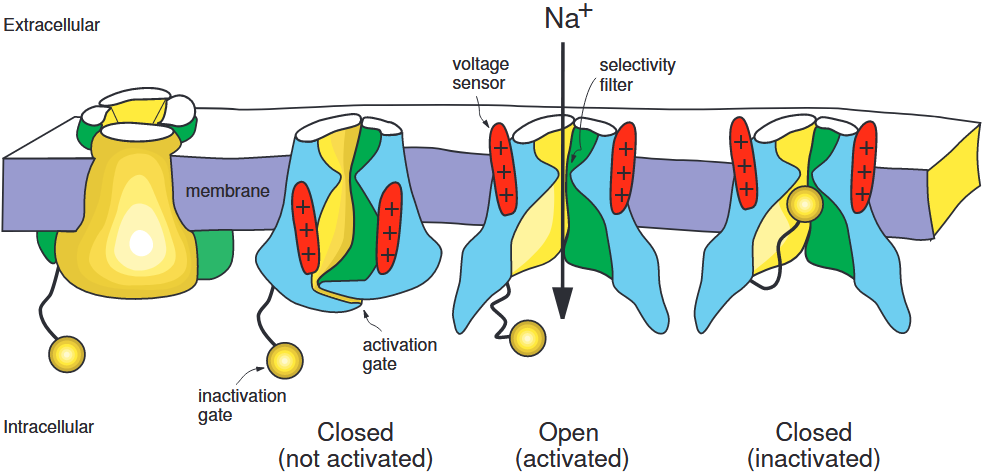
\includegraphics[width=0.85\linewidth]{../img/sleep_and_r5_network/structure_of_v_gated_channels.png}
    \caption[Activation and inactivation gates]{
        \textbf{Activation and inactivation gates.}
        Figure adapted from \cite{izhikevichDynamicalSystemsNeuroscience2006}.
        \textcolor{red}{Text}
    }
    \label{fig:voltage_gated_channel_structure}
\end{figure}

In neuronal models, ion channels are not modelled explicitly. Rather, the models describe the behaviour of a population of ion channels. Thus, the flow of the current through a given channel depends on the maximum conductance (i.e. conductance when all channels are open) and the probability that the gates are in an open state.

Importantly, in response to changes in membrane voltage or ligand concentration, not all channels open or close simultaneously. Instead, transitions between open and closed states occur with a certain probability. At the population level, the probabilistic behaviour is characterised by associated \textbf{gating time constants}. These time constants can vary depending on the channel type, ranging from several milliseconds (fast) to several seconds (slow). The mathematical description of ion channels and their gating mechanisms is provided in \textcolor{red}{Section ???}.


% models
% incorporating ion channels give 

% "Ca-activated potassium channels (K\_Ca2+) are broadly divided into three subtypes based on their
% biophysical and pharmacological profiles: small - (SK), intermediate- (IK) and
% large-conductance (BK) channels" \cite{liuMultipleConductancesCooperatively2008}

% Ca 2 channels comprise two groups: HVA, with activation threshold more positive than approximately
% 30 mV, are further classified into L-, N-, P/Q-, and R-type based on their biophysical and
% pharmacological properties. LVA calcium channels, which activate at potentials more negative
% than approximately 45 mV (Catterall, 2000; Catterall et al., 2005), are traditionally considered
% as T-type Ca 2 channels. \cite{liuMultipleConductancesCooperatively2008}

%%%%%%%%%%%%%%%%%%%%%%%%%%%%%%%%%%%%%%%%%%%%%%%%%%%%%%%%%%%%%%%%%%%%%%%%%%%%%%%%%%%%%%%%
\subsubsection{Known ion channels in \textit{Drosophila} R5 neurons}
There is a limited amount of literature about which ion channels are present in R5 neurons. To my knowledge, the only experimentally confirmed ion channel in these neurons is the T-type $Ca^{2+}$ ion channel, localised at presynaptic terminals (unpublished study by David Owald and colleagues). In many bursting models, T-type channels have been found to be important for bursting due to their kinetic properties (see Section \textcolor{red}{???}).

The second ion channel that potentially is present in R5 neuron is potassium \gls{eag} channel, which could potentially regulate neuronal excitability \cite{bruggemannEtheragogoEncodesVoltagegated1993}. A recent study reported diurnal variation in a gene expression encoding the potassium \gls{eag} channel in R5 neurons of \textit{Drosophila} \cite{doppSinglecellTranscriptomicsReveals2024}. Although direct evidence for the presence of \gls{eag} channels in R5 neurons has not been reported, rhythmic modulation of gene expression suggests that \gls{eag} may indeed be present in R5.

Additionally, voltage-gated sodium ion channels (DMNa$_{\text{v}}$) have been detected in \textit{Drosophila} active neurons, suggesting that they are also expressed in R5 neurons.

Interestingly, both the T-type calcium and DMNa$_{\text{v}}$ channels are encoded by single genes \cite{jeongCaa1TFlyTtype2015,ravenscroftDrosophilaVoltageGatedSodium2020}. \textit{para} gene encoding DMNa$_{\text{v}}$ has been shown to be responsible for mediating both transient and persistent components of sodium channels, likely via a process called alternative splicing \cite{linAlternativeSplicingVoltageGated2009}. To my knowledge, it has never been reported whether alternative splicing applies to the genes encoding T-type and \gls{eag} channels in \textit{Drosophila}.



%%%%%%%%%%%%%%%%%%%%%%%%%%%%%%%%%%%%%%%%%%%%%%%%%%%%%%%%%%%%%%%%%%%%%%%%%%%%%%%%%
\subsection{Sleep in \textit{Drosophila}}

\subsubsection{Circadian and Homeostatic Processes}

Sleep in \textit{Drosophila} is typically defined by a period of inactivity lasting more than 5 minutes \cite{dubowyCircadianRhythmsSleep2017,shaferRegulationDrosophilaSleep2021}. Similar to vertebrates, in \textit{Drosophila} sleep-wake cycle is regulated by two independent processes - circadian and homeostatic \cite{doppSinglecellTranscriptomicsReveals2024,liuSleepDriveEncoded2016}.

Circadian rhythm (circa - approximately, diem - day; also known as process C) refers to the behavioural or physiological processes that recur with a period approximately equal to 24 hours \cite{fernandez-chiappeHighFrequencyNeuronalBursting2021,dubowyCircadianRhythmsSleep2017}. Its function is believed to be the regulation of the sleep-wake cycle and suppression of sleep when sleep is dangerous or unfavourable, even in case of high sleep pressure \cite{shaferRegulationDrosophilaSleep2021,andreaniCircadianProgrammingEllipsoid2022}.
At the cellular level, it consists of transcriptional-translational feedback loops that produce $\sim 24$ hour period cycles in gene expressions, including genes that encode ion-channel proteins
\cite{doppSinglecellTranscriptomicsReveals2024,dubowyCircadianRhythmsSleep2017,andreaniCircadianProgrammingEllipsoid2022}.

On the other hand, homeostasis (or, process S) is thought to reflect the sleep need based on duration of wakefulness, mediated by the build-up of byproducts (e.g. \gls{ros}) from increased neuronal activity
\cite{suarez-grimaltNeuralArchitectureSleep2021,doppSinglecellTranscriptomicsReveals2024,andreaniCircadianProgrammingEllipsoid2022,schmutzSpecificRoleREVERBaControlled2014}. Similar to circadian process, gene expression can also be correlated with the level of the sleep drive \cite{liuSleepDriveEncoded2016}.
R5 neurons, originally referred to as R2 \cite{shaferRegulationDrosophilaSleep2021,liuSleepDriveEncoded2016,donleaRecurrentCircuitryBalancing2018},
consisting of only approximately 32 cells in the adult fly brain \cite{doppSinglecellTranscriptomicsReveals2024}, have been suggested to encode sleep homeostat, as plasticity of these neurons was shown to be both necessary and sufficient for generating sleep drive \cite{liuSleepDriveEncoded2016,doppSinglecellTranscriptomicsReveals2024}.

Interestingly, a recent study reported that a given cell in \textit{Drosophila} was mostly affected by only one process - circadian or homeostatic, with the exception of glial cells, which were affected by both processes \cite{doppSinglecellTranscriptomicsReveals2024}.


%%%%%%%%%%%%%%%%%%%%%%%%%%%%%%%%%%%%%%%%%%%%%%%%%%%%%%%%%%%%%%%%%%%%%%%%
\subsubsection{Circuits involved in \textit{Drosophila} sleep regulation} \label{subsubsec:circuits_in_droso_sleep}

The central complex in \textit{Drosophila} brain has been shown to have a critical function in the regulation of sleep duration and homeostasis. It contains several neuron types, including helicon cells, \gls{dfb}, and \gls{eb} neurons \cite{shaferRegulationDrosophilaSleep2021}.
Generation of coherent \gls{swa} in the central complex has been strongly associated with sleep need and quality \cite{suarez-grimaltNeuralArchitectureSleep2021,raccugliaNetworkSpecificSynchronizationElectrical2019}.
Furthermore, networks within the central complex act as a sensory gate promoting transitions between sleep and wakefulness, similar to mammalian \gls{tc} neurons \cite{raccugliaCoherentMultilevelNetwork2022,gentThalamicDualControl2018}.

\begin{figure}[!b]
    \centering
    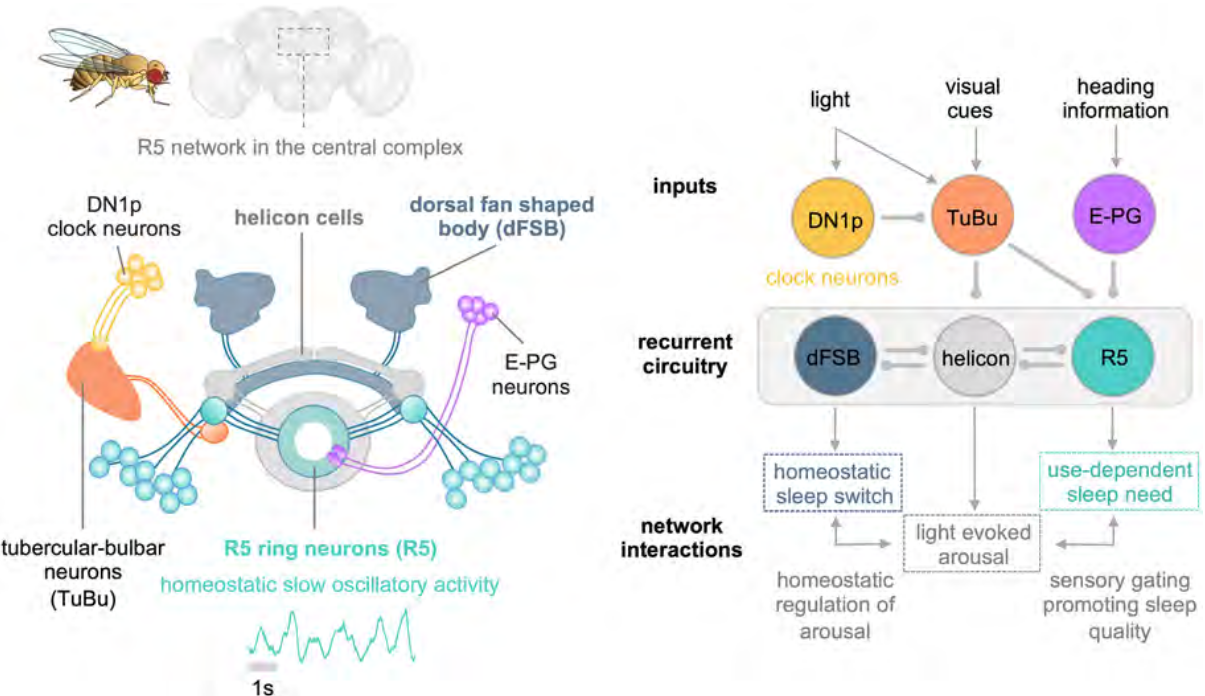
\includegraphics[width=\linewidth]{../img/sleep_and_r5_network/sleep_circuit_suarez.png}
    \caption[Circuits involved in \textit{Drosophila} sleep]{
        \textbf{Circuits involved in \textit{Drosophila} sleep.}
        Left: anatomical organisation of neurons involved in sleep regulation. Right: schematic diagram of sleep-regulating network in \textit{Drosophila} brain.
        Adapted from \cite{suarez-grimaltNeuralArchitectureSleep2021}
        \textcolor{red}{TODO: Replicate image on the right and add connections from R5 to E-PG. Add text to caption}
    }
    \label{fig:droso_sleep_circuit}
\end{figure}

\gls{swa} has been hypothesized to be generated at the level of R5, emerging via synchronous firing of individual R5 neurons at night and following sleep-deprivation \cite{raccugliaNetworkSpecificSynchronizationElectrical2019}.
Studies of the previous decade have identified several circuits modulating R5 activity, sleep-wake states and arousability during sleep. The circuits involved in \textit{Drosophila} sleep regulation are summarised in Figure \ref{fig:droso_sleep_circuit}.

The first circuit involves \gls{dn1p} clock neurons and visually sensitive \gls{tubu} neurons. It represents circadian modulation of R5 neurons through \gls{dn1p} neurons. \gls{tubu} neurons are sensitive to polarised light and are thought to be important for navigation \cite{suarez-grimaltNeuralArchitectureSleep2021}. They provide excitatory input to R5 neurons \cite{duanVisualPathwayCentral2023}. It has been demonstrated that activation of \gls{tubu} neurons increases single-unit power of R5 neurons, induces \gls{swa} in R5 and promotes sleep \cite{andreaniCircadianProgrammingEllipsoid2022,raccugliaNetworkSpecificSynchronizationElectrical2019}. On the other hand, \gls{dn1p} neurons inhibit \gls{tubu} neurons \cite{lamazeWakePromotingCircadianOutput2018} and exhibit diurnal variation in their firing patterns \cite{flourakisConservedBicycleModel2015}. Firing rate of the \gls{dn1p} neurons shows the peak of $\sim 10$ Hz in the early morning, which is monotonically reduced until evening, when the neurons are almost silent. Afterwards, the firing rate starts to gradually increase again until the next morning \cite{flourakisConservedBicycleModel2015}. Thus, \gls{dn1p} mediated inhibition of \gls{tubu} neurons during day might facilitate sensory processing, while release of inhibition in the evening may promote \gls{tubu} mediated compound \gls{swa} in R5 neurons and facilitate switch of their activity from tonic firing to bursting (see Section \ref{subsubsec:transit_tonic_burst}). Indeed, activation of either \gls{dn1p} or \gls{tubu} neurons is sufficient to induce oscillations in R5 neurons \cite{suarez-grimaltNeuralArchitectureSleep2021,raccugliaNetworkSpecificSynchronizationElectrical2019}. Notably, silencing \gls{tubu} neurons did not affect the rebound sleep after sleep deprivation \cite{andreaniCircadianProgrammingEllipsoid2022}, suggesting that they are not involved in homeostatic regulation of sleep.

The second circuit includes functional connection between \gls{dfb} and R5 neurons via excitatory helicon cells \cite{raccugliaCoherentMultilevelNetwork2022}. \gls{dfb} neurons are thought to be sleep-promoting neurons as their activation reduces arousability and induces sleep, while inactivation causes insomnia \cite{pimentelOperationHomeostaticSleep2016,suarez-grimaltNeuralArchitectureSleep2021}. On the other hand, helicon cells respond to visual stimuli \cite{shaferRegulationDrosophilaSleep2021}.

\gls{dfb} neurons are inhibited by wake-promoting dopaminergic neurons \cite{liuTwoDopaminergicNeurons2012}, which mediate dopamine-induced changes within \gls{dfb} neurons, including modulations of passive membrane properties, as well as voltage-dependent and leak potassium conductances \cite{pimentelOperationHomeostaticSleep2016}. Activity of \gls{dfb} neurons changes across the day, with increased activity observed at night \cite{raccugliaCoherentMultilevelNetwork2022}. Similar increase in activity has also been reported during sleep deprivation \cite{pimentelOperationHomeostaticSleep2016}. The increase of the activity in \gls{dfb} has been linked to the activity-dependent accumulation of \gls{ros}. In line with these results, increased activity of these neurons has been reported at night \cite{raccugliaCoherentMultilevelNetwork2022} and following sleep deprivation, whereas they remain silent in rested flies \cite{pimentelOperationHomeostaticSleep2016}. \gls{dfb} neurons inhibit helicon cells, which in turn are interconnected with R5 neurons \cite{suarez-grimaltNeuralArchitectureSleep2021,raccugliaCoherentMultilevelNetwork2022,shaferRegulationDrosophilaSleep2021}.
Thus, reduced activity of \gls{dfb} during daytime might facilitate processing of visual information, while filtering it out at night. As the absence of sensory input may promote synchronisation \cite{raccugliaCoherentMultilevelNetwork2022}, inhibition of helicon cells via \gls{dfb} might induce \gls{swa} in R5 cells.

Apart from the above-mentioned populations, other networks and cell types also have been reported to be involved in \textit{Drosophila} sleep regulation. \gls{mb}, which is involved in olfactory memory, has been shown to contain both wake- and sleep-promoting neurons
\cite{suarez-grimaltNeuralArchitectureSleep2021,dubowyCircadianRhythmsSleep2017}. Furthermore, glial cells, which recently have been shown to integrate both circadian and homeostatic processes \cite{doppSinglecellTranscriptomicsReveals2024}, although the exact function of glia in \textit{Drosophila} sleep regulation is not well-understood. Furthermore,  \glspl{lnv} and \glspl{lnd}, which are clock neurons responsible for, correspondingly, day and evening activity in \textit{Drosophila}, influence the phase of diurnal $Ca^{2+}$ level oscillations in R5 neurons \cite{andreaniCircadianProgrammingEllipsoid2022,liangMorningEveningCircadian2019}.

Interestingly, a recent genetic study which investigated how gene expression levels correlate with circadian and homeostatic processes identified two additional subclusters of \gls{eb} ring neurons, apart from R5, showing a high number of genes correlating with homeostasis \cite{doppSinglecellTranscriptomicsReveals2024}.

Finally, sleep-wakefulness is also potentially regulated by other circuits mediating hunger, sexual arousal, or
social interactions \cite{suarez-grimaltNeuralArchitectureSleep2021,shaferRegulationDrosophilaSleep2021}.


%%%%%%%%%%%%%%%%%%%%%%%%%%%%%%%%%%%%%%%%%%%%%%%%%%%%%%%%%%%%%%%%%%%%%%%%%%%%%%%%%%%%%%%%
\subsubsection{Role of R5 neurons in \textit{Drosophila} sleep} \label{subsubsec:role_of_r5_neurons}

As presented in the previous section, the activity of R5 neurons is modulated by circadian rhythm, homeostatic process, as well as sensory input. This section summarises findings regarding processes and behaviour modulated by R5 neurons, and their role in sleep in \textit{Drosophila}.

Activation of R5 neurons reduces locomotion and increases sleep amount and depth (associated with increased homeostatic sleep drive) even in rested flies \cite{raccugliaCoherentMultilevelNetwork2022,liuSleepDriveEncoded2016}.
However, inactivation of these neurons via inhibition of neurotransmitter release reduced rebound sleep and sleep depth only for sleep-deprived flies, without affecting baseline sleep \cite{liuSleepDriveEncoded2016}.
Additionally, increased expression of \gls{brp} protein, which is important for activity-dependent plasticity, has been reported in R5 neurons following sleep deprivation \cite{liuSleepDriveEncoded2016}.
Notably, such an increase was not observed for other neurons in \textit{Drosophila} brain. Furthermore, among \gls{eb} ring neurons, a high number of genes correlated with sleep drive were found specifically in R5 neurons, while few or none were detected in other \gls{eb} ring neuron clusters \cite{doppSinglecellTranscriptomicsReveals2024}. These suggest that R5 neurons are a central component of the sleep homeostat in \textit{Drosophila}.

It has been suggested that \gls{swa} is generated at the level of R5 neurons \cite{raccugliaNetworkSpecificSynchronizationElectrical2019}, and R5 facilitates \gls{swa} in helicon cells \cite{raccugliaCoherentMultilevelNetwork2022}. Across different species, \gls{swa} have been associated with sleepiness, sleep quality, arousability threshold during sleep, as well as filtering sensory information during sleep \cite{suarez-grimaltNeuralArchitectureSleep2021,raccugliaNetworkSpecificSynchronizationElectrical2019,raccugliaCoherentMultilevelNetwork2022}.
\gls{swa} has been proposed to have same role and effect in \textit{Drosophila}. Furthermore, R5 neurons have been proposed to be functionally similar to \gls{tc} cells in mammals. Similar to \gls{tc} cells, R5 neurons switch their activity pattern from tonic spikes to bursting  with increasing sleep need and following sleep deprivation, promote transition to sleep, and act as a sensory gate, increasing the arousability threshold during sleep while allowing a strong stimulus to induce the behavioural response
\cite{
    suarez-grimaltNeuralArchitectureSleep2021,
    raccugliaNetworkSpecificSynchronizationElectrical2019,
    raccugliaCoherentMultilevelNetwork2022,
    yanSubtypeSpecificRolesEllipsoid2023,
    gentThalamicDualControl2018}.

How can the R5 neuron gate visual information and facilitate the reduction of locomotion? The previous section focused on networks that modulated R5 activity. R5 neurons, in turn, project to helicon and EPG neurons. EPG cells represent the fly's heading direction and are involved in navigation \cite{raccugliaCoherentMultilevelNetwork2022}. They also receive excitation from helicon neurons, whose activation leads to increased activity of EPG neurons and increased locomotion \cite{raccugliaCoherentMultilevelNetwork2022}.
Furthermore, EPG cells were found to be more responsive to visual stimulation during the day in comparison to night \cite{raccugliaCoherentMultilevelNetwork2022}.
Helicon cells also project to EPG neurons. It has been shown that R5 and helicon cells modulate EPG activity in a reciprocal manner: stimulation of helicon cells depolarizes EPG neurons and promotes locomotion, while activation of R5 neurons hyperpolarizes EPG cells and reduces locomotion \cite{raccugliaCoherentMultilevelNetwork2022}. Thus, together with \gls{dfb}, the \gls{dfb}-helicon-R5 network can induce quiescence with increased sleep need by suppressing visual information in helicon cells.
\gls{dfb}-mediated reduction of helicon activity at night could allow R5 neurons to override helicon drive to EPG, thereby reducing its activity and consequently locomotion \cite{raccugliaCoherentMultilevelNetwork2022}.

%%%%%%%%%%%%%%%%%%%%%%%%%%%%%%%%%%%%%%%%%%%%%%%%%%%%%%%%%%%%%%%%%%%%%%%%%%%%%%%%%%%%%%%%
\subsubsection{Circadian and homeostatic regulation of R5 intrinsic properties} \label{subsubsec:circ_and_hemeo_r5}

As stated in the previous section, it is thought that \gls{swa} is generated within \gls{eb} R5 neurons.
Differences between R5 activity during day- and nighttime, as well as following sleep deprivation, might result from circadian and homeostatic regulation, both of the R5 effector circuits, and of R5 neurons themselves. If \gls{swa} is generated at the level of R5 neurons, then when focusing on the R5 network, inputs from effector circuits can be modelled as a constant input current. In this framework, the transition between R5 activity states could be modelled by modulating the magnitude of this input current, in combination with circadian and homeostatic modulations of the intrinsic properties of R5 neurons.

It has been reported that with increased sleep need, R5 neurons show increased firing rate, \cite{raccugliaNetworkSpecificSynchronizationElectrical2019,liuSleepDriveEncoded2016}.
switch from tonic firing to bursting, synchronise and increase delta-power ($0.5$-$1.5$ Hz) \cite{raccugliaNetworkSpecificSynchronizationElectrical2019}. Additionally, the resting membrane potential of R5 neurons has been reported to be more depolarised compared to control animals \cite{liuSleepDriveEncoded2016}. Several studies have reported molecular and cellular changes in R5 neurons in response to elevated sleep pressure.

\textbf{Cytosolic $Ca^{2+}$ concentration.}
Reversible increase in cytosolic $Ca^{2+}$ levels has been observed in \textit{Drosophila} R5 neurons in the morning, evening, and following sleep deprivation \cite{andreaniCircadianProgrammingEllipsoid2022,liuSleepDriveEncoded2016}. Cytosolic $Ca^{2+}$ levels can be modulated by several mechanisms. First, by activation of \glspl{ip3r}, which are intracellular $Ca^{2+}$ channels located on the \gls{er} \cite{schmitzStructuralBasisActivation2022}. \gls{ip3r}-mediated calcium release into cytosol within the cell can, in turn trigger gene expression \cite{schmitzStructuralBasisActivation2022}, and $Ca^{2+}$-dependent synaptic plasticity \cite{liuSleepDriveEncoded2016}. \glspl{ip3r} regulation itself has been hypothesised to play a role in circadian clock entrainment in mammals \cite{hamadaRoleInositolTrisphosphateinduced1999}. Second, cytosolic $Ca^{2+}$ levels can also be increased by activation of $Ca^{2+}$ channels. It has been shown that T-Type $Ca^{2+}$ channels that are present in \textit{Drosophila} presynaptic terminals are more active during the night in comparison to day (private discussion with David Owald).
Thus, increased neuronal activity during night and sleep deprivation could also explain the rise in cytosolic $Ca^{2+}$ levels. To my knowledge, whether the increase in calcium concentration is a cause or a consequence of increased neuronal activity and bursting in R5 neurons is unknown. However, both processes might modulate cytosolic $Ca^{2+}$ level in \textit{Drosophila} R5 neurons.

\textbf{Gene expression.}
Expression of the gene encoding potassium \gls{eag} channel has been observed to negatively correlate with sleep drive in R5 neurons \cite{doppSinglecellTranscriptomicsReveals2024}. Taking into account that $K^{+}$ currents hyperpolarise the membrane, an elevated number of \gls{eag} channels may oppose depolarising currents, thereby reducing excitability and preventing transition to the bursting state.

\textbf{Modulation within presynaptic terminals.}
Furthermore, \gls{brp} levels have been reported to increase only in R5 neurons following sleep deprivation \cite{liuSleepDriveEncoded2016}. \glspl{brp} are localized at presynaptic terminals \cite{waghBruchpilotProteinHomology2006}, and elevated \gls{brp} level has been associated with promotion of high-voltage activated $Ca^{2+}$ channel density \cite{kittelBruchpilotPromotesActive2006}. Strikingly, neither morning nor evening sleep deprivation induced considerable changes in gene expression \cite{andreaniCircadianProgrammingEllipsoid2022}. These results may reflect a process called synaptic remodelling, where existing synapses are eliminated to form new synapses on different dendritic or axonal branches \cite{kurupNeuralCircuitRewiring2016}. Alternatively, this absence of the effect may have been influenced by experimental conditions or methodological limitations.


%%%%%%%%%%%%%%%%%%%%%%%%%%%%%%%%%%%%%%%%%%%%%%%%%%%%%%%%%%%%%%%%%%%%%%%%%%%%

\subsection{Bursting}

\subsubsection{Onset and offset of bursts}

Bursting in neurons is characterised by transition of the neuron between two states: 1) resting state, where the neuron does not fire action potentials and 2) spiking state (Fig. \ref{fig:ionic_basis_for_slow_fast_bursting}, bottom). Over the time course, the bursting neuron switches between the two states, resulting in the periods of quiescence (i.e. inactivity, or resting) and high-frequency spiking.

Generally, bursting involves an interplay between oscillations with fast and slow timescales. Fast time scale is related to the spiking within a burst, while the slow timescale is associated with modulation of the transition between spiking and resting states \cite{izhikevichDynamicalSystemsNeuroscience2006}. What cellular mechanisms cause burst initiation and termination? These mechanisms can generally be divided into four classes based on the underlying processes responsible for burst initiation and termination, as summarised by Izhikevich \cite{izhikevichDynamicalSystemsNeuroscience2006} (see also Figure \ref{fig:ionic_basis_for_slow_fast_bursting}). In the following, the main principles behind these mechanisms will be outlined.

\begin{figure}[!t]
    \centering
    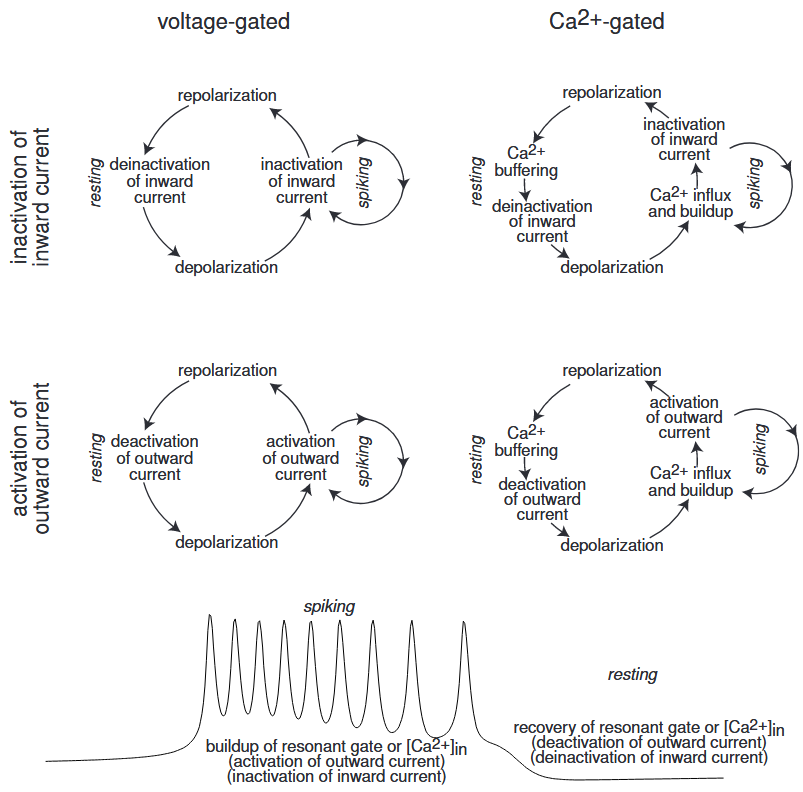
\includegraphics[width=0.85\linewidth]{../img/modelling_r5/examples/bursting_ionic_basis.png}
    \caption[Cellular mechanisms of burst generation]{
        \textbf{Cellular mechanisms of burst generation.}
        For the details see the main text.
        Figure adapted from \cite{izhikevichDynamicalSystemsNeuroscience2006}, with modifications.
        \textcolor{red}{Detailed Text}
    }
    \label{fig:ionic_basis_for_slow_fast_bursting}
\end{figure}

Mechanism of the burst termination might involve either voltage and/or $Ca^{2+}$ dependent hyperpolarising currents.
The onset and offset of the spiking phase can be caused by inward and/or outward currents. Inward currents are depolarising currents (mostly mediated by sodium ($Na^+$) and calcium ($Ca^{2+}$) ions) driving the membrane potential towards the spiking threshold. Outward currents, on the other hand, are hyperpolarising currents, effectively increasing spiking threshold and are mostly mediated by potassium ($K^+$) ions.
The onset (offset) of the burst can thus be caused by deinactivation (inactivation) of inward currents, or deactivation (activation) of outward currents. Deinactivation of inward currents requires the corresponding ion channel to have an inactivation gate, and deinactivation refers to the removal of inactivation, i.e. opening of the inactivation gate.

Furthermore, the termination of a burst can be caused by ion channels which mediate hyperpolarising currents and whose activation depends on the intracellular calcium concentration. Calcium entry can lead to activation of $Ca^{2+}$-dependent outward currents, or inactivation of $Ca^{2+}$-dependent inward currents. This, in turn, promotes the dominance of outward currents, driving the membrane to more negative values and thus contributing to spike termination.

Within the scope of the current thesis it is investigated whether bursting for \textit{Drosophila} R5 neurons depends on T-type $Ca^{2+}$ channels. The bursting mechanism mediated by T-type channels will be discussed in more detail in Section \ref{subsubsec:ion_channel_contributions}. Shortly, in bursting models, where onset and offset of the bursts are mediated by T-type channels, the transition between spiking and resting states occurs, correspondingly, via deinactivation and inactivation of these channels (upper left diagram in Figure \ref{fig:ionic_basis_for_slow_fast_bursting}).


%%%%%%%%%%%%%%%%%%%%%%%%%%%%%%%%%%%%%%%%%%%%%%%%%%%%%%%%%%%%%%%%%%%%%%%%%%%%%%%%%%%%%%%%
\subsubsection{Ion channel contributions in bursting and under sodium channel blockade} \label{subsubsec:ion_channel_contributions}

Although the cellular basis has been investigated in \textit{Drosophila} R5 neurons, and also little is known about ion channels expressed in these neurons, numerous experimental and computational studies have investigated the effects of ion channels in burst generation in other neuronal types in various animal species. These include \glspl{lnv} neurons in \textit{Drosophila}, as well as bursting neurons in rodents \cite{vickstromTTypeCalciumChannels2020,golombContributionPersistentNa2006,liuMultipleConductancesCooperatively2008,wangMultipleDynamicalModes1994,mccormickModelElectrophysiologicalProperties1992} Understanding bursting mechanism of other models might provide an insight which ion channels might contribute to burst firing in \textit{Drosophila} R5 neurons. The following section summarises ion channels reported to contribute to bursting activity and describes their roles in shaping the burst dynamics.

\noindent\textbf{T-Type and HCN channels}

T-Type and \gls{hcn} channels have been found to be important components for many bursting neurons in various animal species \cite{amarilloInterplaySevenSubthreshold2014,vickstromTTypeCalciumChannels2020,destexheModelInwardCurrent1993},
and taking part in subthreshold dynamics and slow oscillations \cite{wangMultipleDynamicalModes1994}.
They have been hypothesised and experimentally validated to play a substantial role in mediating bursting and low-threshold $Ca^{2+}$ spikes after sodium channels are blocked in the experimental conditions.
T-Type channels are voltage-gated calcium channels characterised by fast low-voltage activation, inactivate slowly at potentials larger than the firing threshold and deinactivate at hyperpolarised membrane potentials. Generally, \gls{hcn} channels have only an activation gate that opens with hyperpolarisation, mediates depolarising current \cite{destexheModelInwardCurrent1993}, and facilitates setting the minimal membrane potential (e.g. during oscillations) at more depolarised potentials \cite{liuMultipleConductancesCooperatively2008}.

% TODO: Maybe add another literature in "see e.g. described previously"
The mechanism for bursting that is mediated by T-type- and h-currents has been described previously (see e.g. \cite{liuMultipleConductancesCooperatively2008}). In these models, hyperpolarising current activates \gls{hcn} channels that, once opened, depolarise the membrane until the activation threshold of T-type channels. When T-type channels open, they provide an excitatory current driving the neuron into a spiking state.
At higher potentials, T-type currents slowly inactivate, and once inactivation is sufficiently large, the hyperpolarising currents take over to drive the membrane potential back to a hyperpolarised state.
Here, T-type channels deinactivate and \gls{hcn} channels activate, and the cycle repeats. Such bursting, when a neuron bursts due to hyperpolarising current, is referred to as \textbf{inhibition-induced bursting} \cite{izhikevichDynamicalSystemsNeuroscience2006}.

It is worth noting that \gls{hcn} current is not necessary for inhibition-induced bursting. For example, within the scope of this thesis, simulations of the bursting model described in \cite{wangMultipleDynamicalModes1994}
showed that for this model, persistent sodium, leak, potassium and T-type channels are necessary and sufficient to induce bursting behaviour.

H current has been shown to increase burst frequency \cite{liuMultipleConductancesCooperatively2008,mccormickModelElectrophysiologicalProperties1992}.
Furthermore, it has also been associated with \gls{ahp} (undershoot of membrane potential below resting membrane potential \cite{mccormickModelElectrophysiologicalProperties1992}, e.g. Figure \ref{fig:sleep_r5_knock_ttx_voltage} top right plot). For example, \textcolor{red}{citation} reported reduction and abolishment of \gls{ahp} amplitude with increasing blockade of \gls{hcn} channels. However, \gls{hcn} is not necessary to observe \gls{ahp}. Rather, the undershoot depends on the dynamical properties of the system, as it will be discussed in more detail in \textcolor{red}{Section ???}.

\noindent\textbf{L-Type channels}

Another $Ca^{2+}$ channel that could be involved in bursting are the L-type channels. Similar to T-type channels, they are characterised by slow inactivation, however, they are activated at higher membrane potentials \cite{liuMultipleConductancesCooperatively2008}.
These channels have been shown to mediate \gls{lva} $Ca^{2+}$ currents and increase the burst duration in mice periglomerular cells \cite{liuMultipleConductancesCooperatively2008} and \textit{Drosophila} motoneurons \cite{kadasDendriticAxonalLType2017}.
Although it is not yet known whether \textit{Drosophila} R5 neurons express L-type channels, they are potential candidates for involvement in the modulation of bursting in these cells.


\noindent\textbf{Sodium channels}

Persistent sodium channels have been shown to modulate the number of spikes within a burst. Specifically, for several computational and biological models, increasing the maximal conductance of these channels increased the number of spikes per burst \cite{liuMultipleConductancesCooperatively2008,golombContributionPersistentNa2006}.

As bursting with one spike per burst can be thought of as tonic firing, modulation of persistent sodium channels can be a potential mechanism to switch from tonic to bursting behaviour in \textit{Drosophila} R5 neurons.

\noindent\textbf{Potassium channels}

As in neurons reversal potential of generally is generally found to be at much negative potentials than the resting membrane potential (see e.g. Table \ref{tab:typical_ion_concentrations_in_mammaly}), they generally counteract depolarising currents and result in reduction of neuronal response to such currents \cite{mccormickModelElectrophysiologicalProperties1992}. Depending on their activation threshold and dynamic properties, they can influence subthreshold and/or spiking activity. For example, transient potassium current has been proposed to modulate the initial phase of \gls{lva} calcium spikes \cite{huguenardSimulationCurrentsInvolved1992} and reduce the firing rate of a neuron \cite{mccormickModelElectrophysiologicalProperties1992}. In contrast, another voltage-gated potassium current, characterized by slower activation and inactivation kinetics (correspoding ionic current referred to as $I_{K2}$), has been suggested to influence the later phases of \gls{lva} $Ca^{2+}$ spikes \cite{huguenardSimulationCurrentsInvolved1992}, while also contributing to decreased neuronal firing rate \cite{mccormickModelElectrophysiologicalProperties1992}.

Another important potassium channel is the large-conductance $Ca^{2+}$ activated potassium channel (referred to as the BK channel). Activation of these channels may require simulations of depolarisation and calcium influx. Due to their large conductance, it has been proposed that BK channels might contribute to the termination of the burst, thus regulating the burst
duration \cite{liuMultipleConductancesCooperatively2008}.

\noindent\textbf{Leak Channels}

Leak channels predominantly modulate resting membrane potential \cite{mccormickModelElectrophysiologicalProperties1992,amarilloInterplaySevenSubthreshold2014}. The parameters for these channels (maximal conductance and reversal potential) are often tuned to reproduce experimentally observed resting membrane potential and input resistance \cite{wangMultipleDynamicalModes1994}.
% TODO: Is WANG correct citation????

Of note, intra- and extracellular $Ca^{2+}$ concentration has been shown to also modulate bursting behaviour. While intracellular calcium buffering has been shown to stabilise bursting activity, as well as resting membrane potential \cite{liuMultipleConductancesCooperatively2008}, decreasing extracellular $Ca^{2+}$ concentration can switch from spiking to bursting activity \cite{golombContributionPersistentNa2006}.

\vspace*{0.5cm}

How can a neuron switch from tonic to bursting activity? As it was stated above, modulation of the number of persistent sodium channels (which will affect the maximal conductance at the population level), as well as a decrease in extracellular calcium concentration, can induce bursting. It has been demonstrated that the same could be achieved by modulation of maximal voltage-gated transient- and calcium-gated potassium channels \cite{franciRobustTunableBursting2018}. Generally, as potassium channels modulate the excitability of the cell, switching from bursting to tonic activity could potentially be achieved by increasing the maximal conductance of other voltage-gated potassium channels. However, it is important to note,
that this might not be straightforward, as computational study of McCormick and Huguenard showed that in their model decrease in any of the voltage-dependent potassium currents increased other voltage-gated potassium currents \cite{mccormickModelElectrophysiologicalProperties1992}.

\vspace*{0.5cm}

It is important to keep in mind that R5 neurons do not exhibit inhibition-induced bursting, and neither hyperpolarisation-activated depolarising currents are involved in bursting activity. To my knowledge, there is no published experimental observation regarding this matter.

Secondly, even if the bursts in R5 neurons are mediated by T-type channels, the contribution of specific ion channels might depend on the properties of the whole dynamical system. Several examples will be presented in the following.

It has been shown that elevated maximal conductance of T-type channels increases burst duration and decreases period of bursting \cite{parkMathematicalModelSubthalamic2021}. Furthermore, the maximal conductance of those channels has been reported to positively correlate with the resting membrane potential \cite{amarilloInterplaySevenSubthreshold2014}. However, the model presented in \cite{amarilloInterplaySevenSubthreshold2014} did not contain calcium-gated potassium channels. Because the latter mediates hyperpolarising current, a reduction in the influx of calcium through calcium channels might induce reduced activation of such potassium channels. This might effectively lead to an increase in resting membrane potential instead of a decrease expected due to the depolarising nature of T-type currents.

Furthermore, although for some models persistent sodium channels are necessary to induce bursting (see e.g. \cite{liuMultipleConductancesCooperatively2008,wangMultipleDynamicalModes1994}), for other models these channels are neither necessary nor sufficient to induce bursting (see e.g. \cite{golombContributionPersistentNa2006}).

Such differences in modulatory effects can be observed not only between different models but also within the same model operating in different parameter regimes. For example, altering a single parameter may result in an increase or decrease in the number of spikes per burst, depending on the values of the chosen fixed parameters.

% Paper about M-Type current mediated bursts. Paper about Drosophila removing T-Type channels,
% but here the burst freqeucny was more or less same. And another paper, with bursting being
% changed.

% Another current which may be important for bursting is L type current (paper in drosophila).

% Other channels, like Na, Potassium, Leak.

% Importantly, these depends on general set of the ion channels as well as operating regimes.
% Example from that paper where positive/negative correlation depended on gC.


% small LNvs (sLNvs) are bursting neurons, and Ih is necessary to achieve the high-frequency bursting firing pattern
% characteristic of both types of LNvs in females.
% \cite{fernandez-chiappeHighFrequencyNeuronalBursting2021} (Fernandez-Chiappe et al 2021)


% However, this is not very helpful, as the bursting dpends on the gating properties and
% time constants of the ion channels. Many different systems can burst, including
% minimual models of bursting (izhikevich). Furthermore, undershoot does not
% necessarily mean h-current, but could be explained with dynamical properties
% of the system, even without h-current (see section XXX).


%%%%%%%%%%%%%%%%%%%%%%%%%%%%%%%%%%%%%%%%%%%%%%%%%%%%%%%%%%%%%%%%%%%%%%%%%%%%%%%%%
\subsection{Experimental Findings and Mechanistic Proposals}

\subsubsection{\texorpdfstring{Blocking of $Na$ and T-Type $Ca^{2+}$ Channels in R5 Neurons}{Blocking of Na and T-Type Ca2+ Channels in R5 Neurons}}

T-Type $Ca^{2+}$ channels have been shown to mediate bursting activity in many neurons, regardless of animal species (see Section \ref{subsubsec:ion_channel_contributions}), including mammalian \gls{tc} cells.  \textit{Drosophila} homologe for mamallian T-Type $Ca^{2+}$ channels has also been identified \cite{jeongCaa1TFlyTtype2015}.
As correspondence between R5 and \gls{tc} cells has been suggested, a natural question to ask would be whether and to what extent T-Type channels contribute to bursting in \textit{Drosophila} R5 neurons.

\begin{figure}[!t]
    \centering
    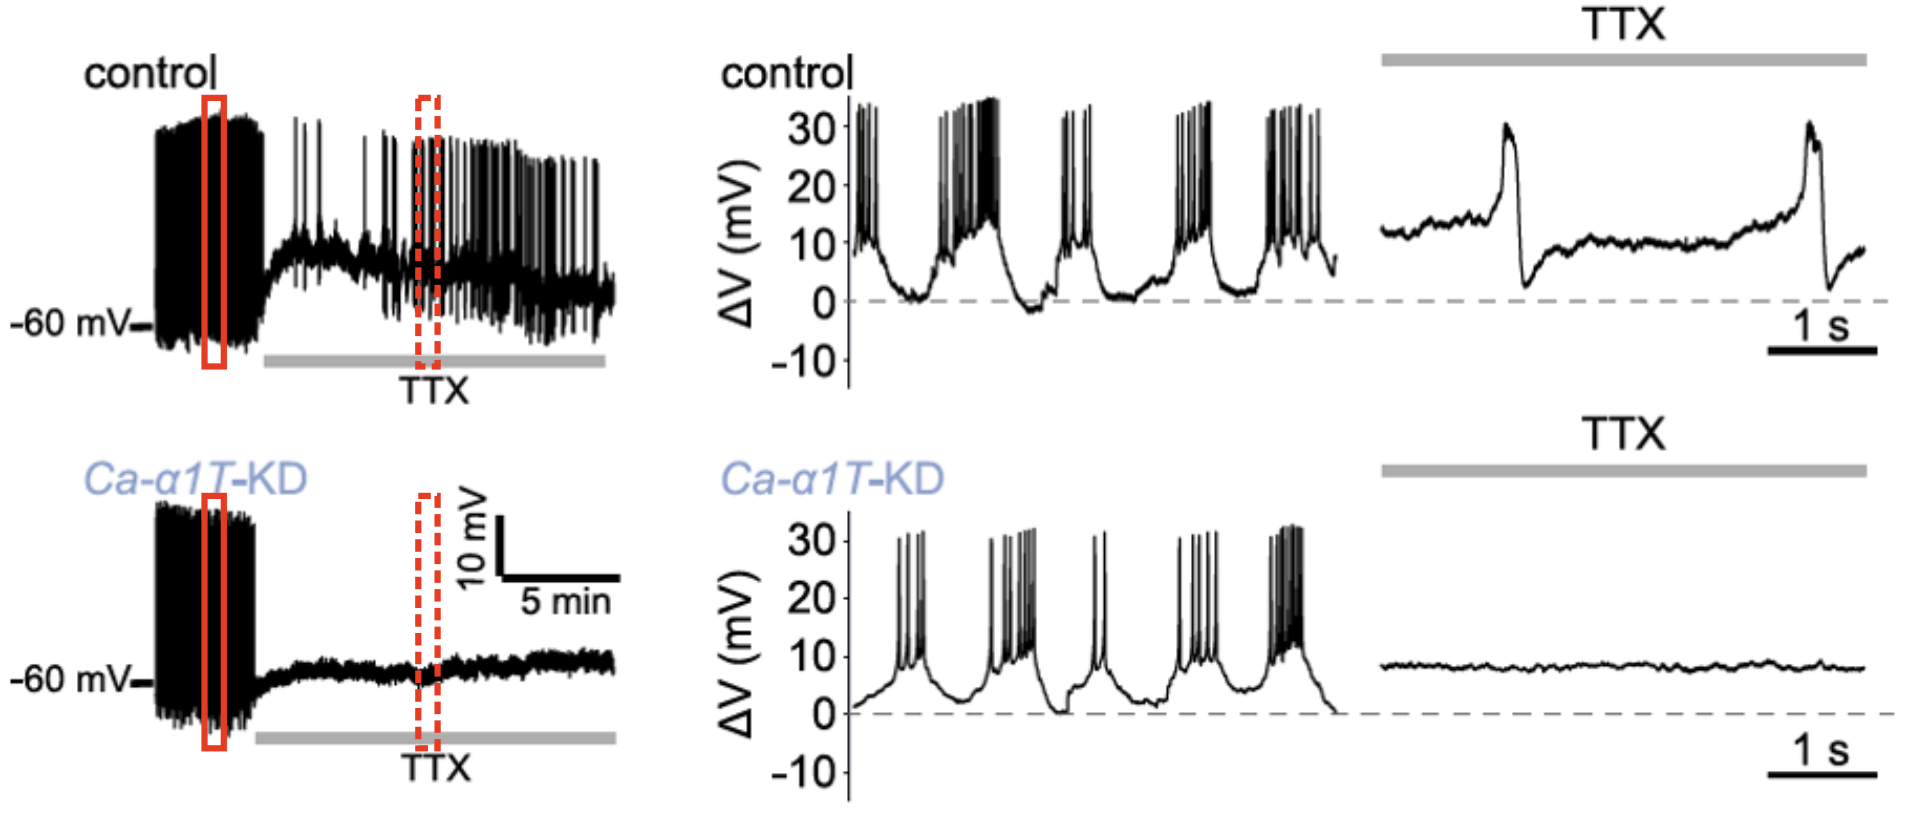
\includegraphics[width=0.95\linewidth]{../img/sleep_and_r5_network/CaaT_knock_and_ttx/voltage_traces_labelled.png}
    \caption[Voltage traces in control and $Ca\text{-}\alpha1T\text{-KD}$ flies following block of sodium channels]{
        \textbf{Voltage traces in control and $\bm{Ca\text{-}\alpha1T\text{-KD}}$ flies following block of sodium channels.}
        Left: recorded voltage traces obtained by \textcolor{red}{patch-clamp} recordings of R5 neurons from \textcolor{red}{sleep-deprived} control (top) and T-Type channel knockdown (bottom) flies.
        Middle: Recorded voltage traces from the region outlined by the solid red rectangle in the left plots (before application of \gls{ttx}); \textcolor{red}{$0$ on the $\Delta V$ axis accounts for the mean resting membrane potential (+ corrected for Liquid Junction Potential (?) Maybe that is why in contrast to Figure \ref{fig:sleep_r5_knock_ttx_frequencies}) the trough on the left plot seems to be lower for $Ca-\alpha1T-KD$ than for control.}Right: Recorded voltage traces from the region outlined by the dashed red rectangle in the left plots (after application of \gls{ttx}). The image displays unpublished data provided by David Owald and Anatoli Ender.
    }
    \label{fig:sleep_r5_knock_ttx_voltage}
\end{figure}

\begin{figure}[!t]
    \centering
    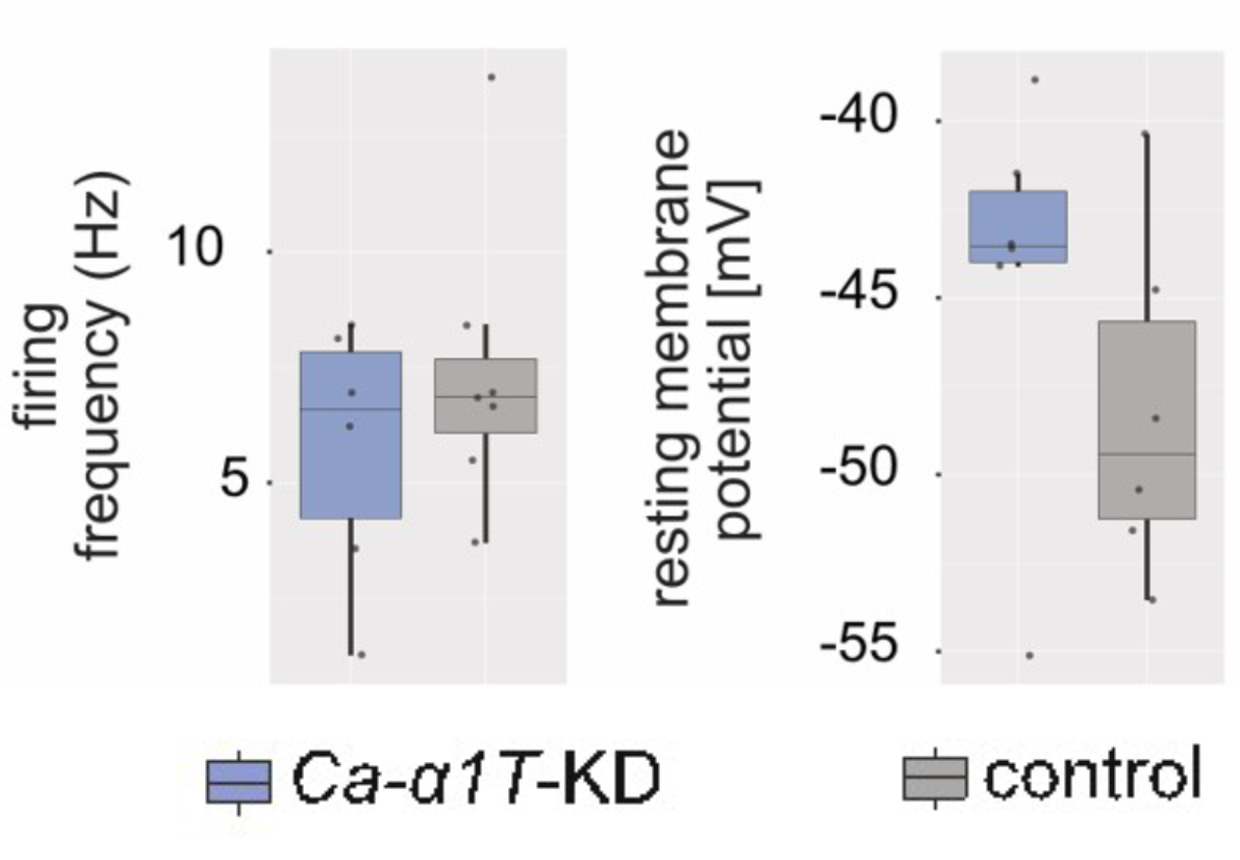
\includegraphics[width=0.5\linewidth]{../img/sleep_and_r5_network/CaaT_knock_and_ttx/frequencies_whole.png}
    \caption[Firing rate and resting membrane potential after $Na$\textsuperscript{+} block in control and $Ca\text{-}\alpha1T\text{-KD}$ flies]{
        \textbf{Firing rate and resting membrane potential after Na\textsuperscript{+} block in control and $\bm{Ca\text{-}\alpha1T\text{-KD}}$ flies.}
        Comparison of firing rate and resting membrane potential between T-Type channel knockdown and control flies before \gls{ttx} application. The corresponding voltage traces are given in Figure \ref{fig:sleep_r5_knock_ttx_voltage}.
        The image displays unpublished data provided by David Owald and Anatoli Ender.
    }
    \label{fig:sleep_r5_knock_ttx_frequencies}
\end{figure}

An unpublished study by \textcolor{red}{David Owald and Anatoli Ender} has revealed that T-Type channels in R5 neurons are expressed at presynaptic sites.
% \textcolor{red}{(There was a paper about similar model for TC cells by Destexhe I guess.)}
Patch-clamp recordings from R5 neurons of sleep-deprived flies exhibited bursting activity (Figure \ref{fig:sleep_r5_knock_ttx_voltage} top). Blocking $Na$ channels with \gls{ttx} resulted in oscillations with pronounced \gls{ahp} and lower frequency (\textcolor{red}{exact value}) in comparison to $1$ Hz interburst frequency (defined by time period between first spike in the current burst and last spike in the preceding burst) before \gls{ttx} application (Figure \ref{fig:sleep_r5_knock_ttx_voltage}, top).

Next, using genetic tools, Owald and colleagues knocked down T-type calcium channels in \textit{Drosophila} R5 neurons (labelled as $Ca$-$\alpha$1$T$-KD flies) (Figure \ref{fig:sleep_r5_knock_ttx_voltage}, bottom). Interestingly, T-Type $Ca^{2+}$ \gls{kd} fly R5 neurons still retained bursting activity, with the same intraburst frequency (frequency of the spikes within burst, Figure \ref{fig:sleep_r5_knock_ttx_frequencies}, left). Strikingly, the resting membrane potential was higher for $Ca$-$\alpha$1$T$-KD flies in comparison to the control ones. At first sight, this result seems counterintuitive, as $Ca^{2+}$ currents are depolarizing currents (rising membrane potential towards spiking threshold). Indeed, simulation studies of \gls{tc} cells have reported a reduction in resting membrane potential following the blockade of T-Type $Ca^{2+}$ channels \cite{amarilloInterplaySevenSubthreshold2014}.
$Ca$-$\alpha$1$T$-KD flies oscillatory activity diminished after \gls{ttx} application, suggesting a role for the T-type calcium current in generating those oscillations.

Why is bursting retained, and why increase in resting membrane potential is observed with after T-Type $Ca^{2+}$ channel blockade remains unknown. One possible explanation for the retention of bursting activity is that a subset of T-type channels may remain functional after $Ca$-$\alpha1T$ knockdown. The remaining calcium current could be sufficient to depolarize the membrane potential to the spiking threshold and support bursting, however, insufficient to sustain oscillatory activity following $Na$ channel blockade. Alternatively, other ion channels that conduct depolarizing currents might contribute to bursting. A potential candidate is \gls{hva} $Ca^{2+}$ current mediated by L-type calcium channels. As described in Section \ref{subsubsec:ion_channel_contributions}, L-type channels are characterized by slow inactivation, similar to the T-type $Ca^{2+}$ channels. Thus, instead of T-type channels, bursting can potentially be mediated by L-type channels.

As discussed in Section \ref{subsubsec:ion_channel_contributions}, an increase in resting membrane potential following blockade of T-type $Ca^{2+}$ channels might be an indication of the calcium-gated potassium channels. If the conductance of these potassium channels is larger than that one for the T-type channel, elimination of T-type channels may
effectively cause an increase in resting membrane potential via weaker activation of $Ca^{2+}$-gated $K^+$ channels. Alternatively, this could be the result of a more complex mechanism, mediated by $Ca^{2+}$-dependent synaptic plasticity.


%%%%%%%%%%%%%%%%%%%%%%%%%%%%%%%%%%%%%%%%%%%%%%%%%%%%%%%%%%%%%%%%%%%%%%%%%%%%%%%%%%%%%%%%%%
\subsubsection{Transition between tonic and bursting activity} \label{subsubsec:transit_tonic_burst}

\begin{figure}[!b]
    \centering
    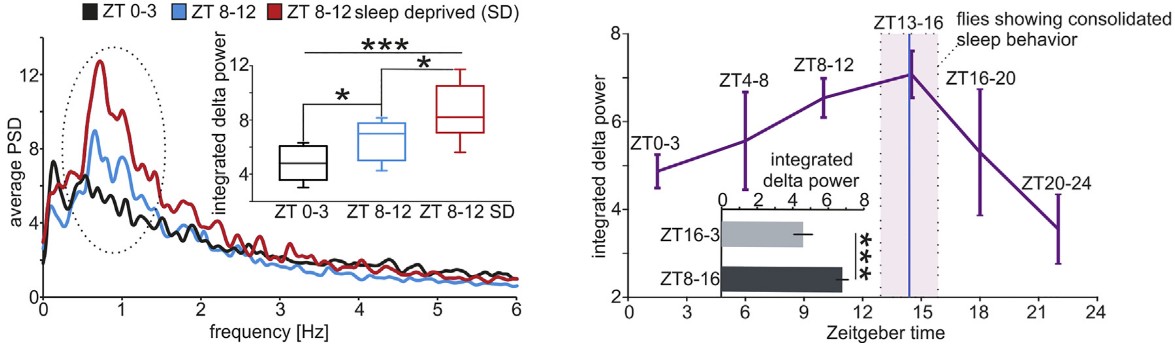
\includegraphics[width=0.95\linewidth]{sleep_and_r5_network/raccuglia_compound_delta.png}
    \caption[Diurnal variation of R5 compound \gls{swa} power spectrum]{
        \textbf{Diurnal variation R5 compound \gls{swa} power spectrum}.
        Adapted from \cite{raccugliaNetworkSpecificSynchronizationElectrical2019}
        \textcolor{red}{TODO: Text}
    }
    \label{fig:raccuglia_compound_delta_oscillations}
\end{figure}

\begin{figure}[!b]
    \centering
    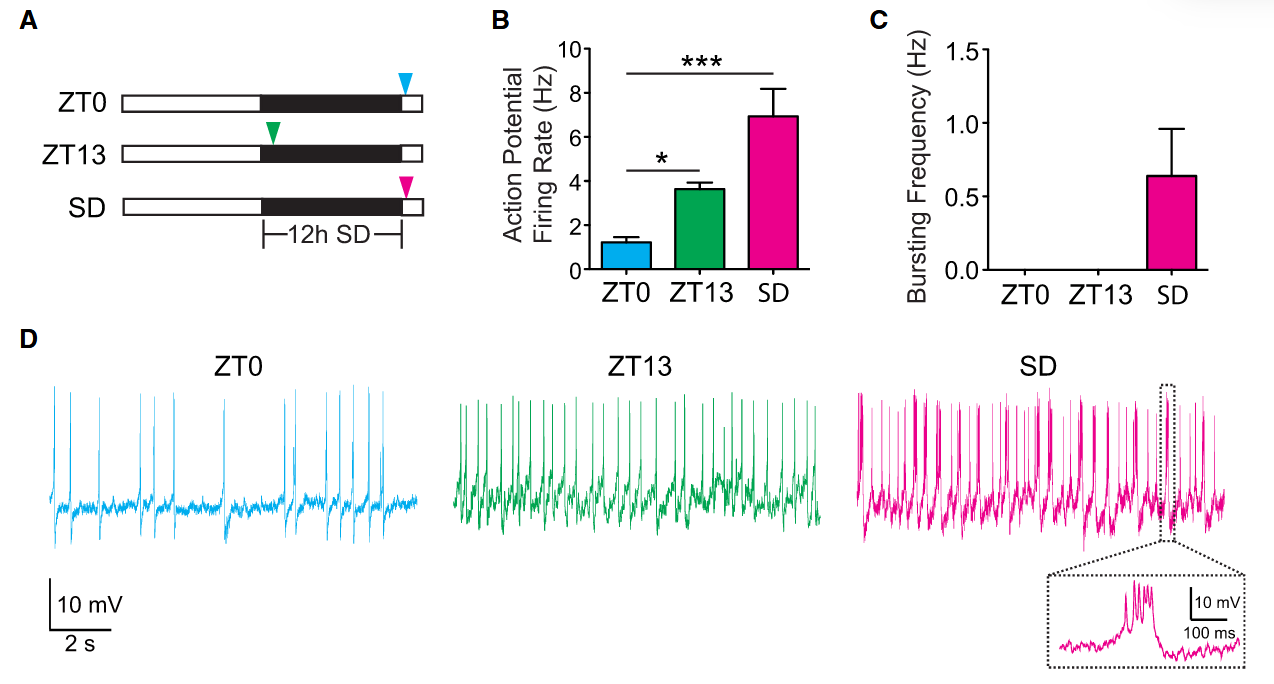
\includegraphics[width=0.95\linewidth]{tmp/freuqnecy_vs_time.png}
    \caption[Diurnal variation of R5 single-cell voltage trace.]{
        \textbf{Diurnal variation of R5 single-cell voltage trace.}.
        Adapted from \cite{liuSleepDriveEncoded2016}
        \textcolor{red}{TODO: Text}
    }
    \label{fig:tmp_frequency_vs_zt}
\end{figure}

R5 neurons synchronize and exhibit bursting activity with increasing sleep need \cite{raccugliaNetworkSpecificSynchronizationElectrical2019,liuSleepDriveEncoded2016}
(Figures \ref{fig:raccuglia_compound_delta_oscillations}-\ref{fig:tmp_single_unit_r5_day_night}).
Study of Raccuglia and colleagues showed that delta power ($0.5$-$1.5$Hz) of compound R5 oscillations increases progressively throughout the day, peaks during the night when the fly displays consolidated sleep, and subsequently declines toward the morning \cite{raccugliaNetworkSpecificSynchronizationElectrical2019} (Figure \ref{fig:raccuglia_compound_delta_oscillations} right).
The delta power of compound \gls{swa} was observed to be even stronger for sleep-deprived flies (Figure \ref{fig:raccuglia_compound_delta_oscillations} left). Furthermore, Liu and colleagues reported an increase in action potential firing rate of R5 neurons at early night, in comparison to early morning \cite{liuSleepDriveEncoded2016}, and highest for sleep-deprived flies (Figure \ref{fig:tmp_frequency_vs_zt}). Of note, interestingly, they observed bursting in R5 neurons only in sleep-deprived flies (\textcolor{red}{see also Section ??? - Discussion}).

The compound $\sim 1$ Hz \gls{swa} in R5 originates from the synchronization between individual R5 units, which display a similar peak in the power spectrum as observed in compound oscillations \cite{raccugliaNetworkSpecificSynchronizationElectrical2019} (Figure \ref{fig:tmp_single_unit_r5_day_night}).
In contrast, during daytime, the peak in the delta power is observed neither in the compound \gls{swa} (Figure \ref{fig:raccuglia_compound_delta_oscillations} left) nor in the single-cell activity (Figure \ref{fig:tmp_single_unit_r5_day_night} left).
Furthermore, during the day, the R5 neurons exhibit tonic firing rate (Figure \ref{fig:tmp_frequency_vs_zt}).

\begin{figure}[!t]
    \centering
    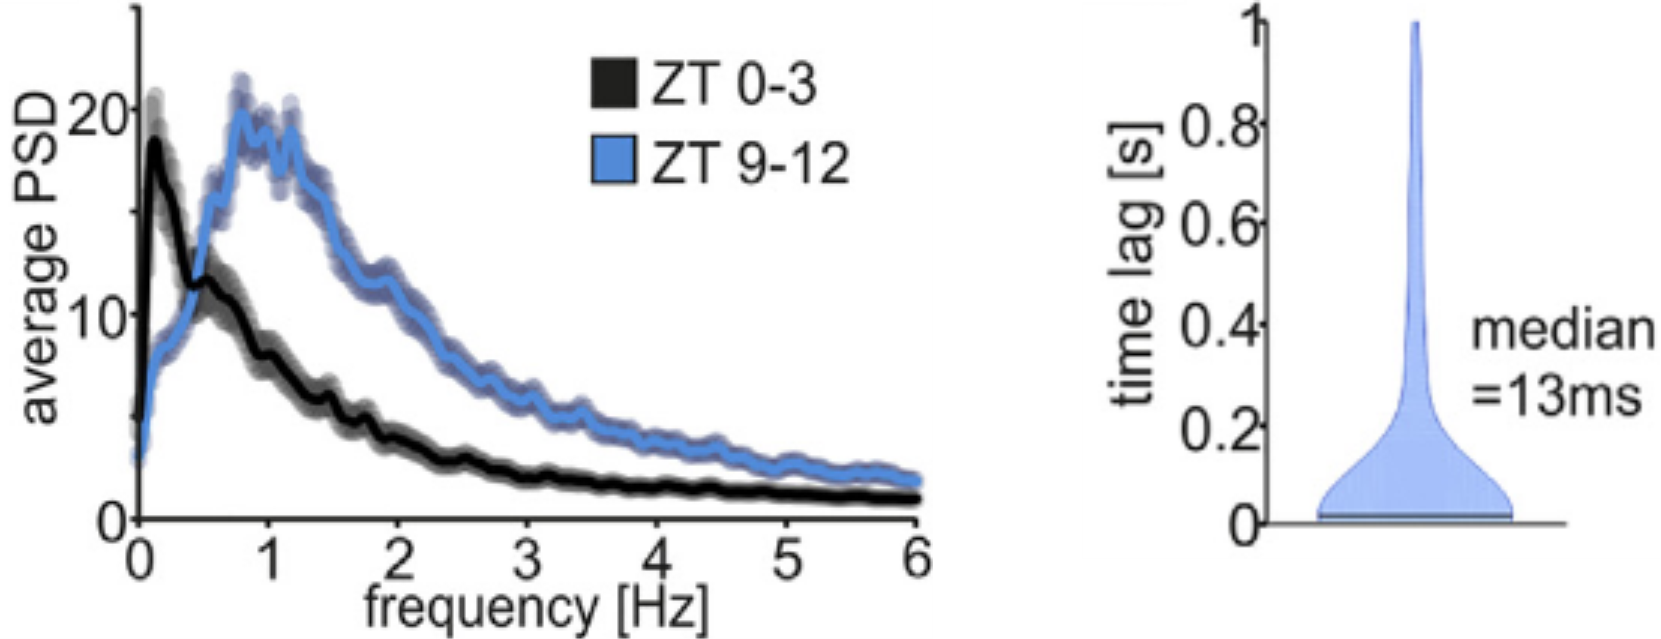
\includegraphics[width=0.7\linewidth]{tmp/raccuglia_2019_single_unit_sync.png}
    \caption[Contribution of individual R5 neurons in compound \gls{swa}]{
        \textbf{Contribution of individual R5 neurons in compound \gls{swa}}
        Left: Average power spectrum of R5 single-cell \gls{swa}.
        Right: Pair-wise time lag distribution of depolarization phases between individual R5 neurons recorded at \gls{zt} 9-12.
        Adapted from \cite{raccugliaNetworkSpecificSynchronizationElectrical2019}
        \textcolor{red}{TODO: Text}
    }
    \label{fig:tmp_single_unit_r5_day_night}
\end{figure}

Transition from tonic to bursting activity, and increased power in the compound \gls{swa} has been associated with reduced locomotion, increased sleep drive, sleep depth, and filtering of the sensory information during sleep
\cite{liuSleepDriveEncoded2016,raccugliaNetworkSpecificSynchronizationElectrical2019,
raccugliaCoherentMultilevelNetwork2022,suarez-grimaltNeuralArchitectureSleep2021}.
However, how individual R5 neurons switch from tonic spiking to bursting is not well understood.

Generally, the neurons which exhibit inhibition-induced bursting can fire tonically if an excitatory current is injected (see e.g. \cite{wangMultipleDynamicalModes1994}).
In the case of excitatory drive, the neuron is driven in the spiking state by the constant input current, rather than via T-type $Ca^{2+}$ channels. However, for R5 neurons, the switch from bursting to tonic activity cannot be explained solely by a change in external drive, as they do not exhibit high-frequency tonic spikes during the daytime.

As discussed in Section \ref{subsubsec:circ_and_hemeo_r5}, this change in activity can be caused by several factors. First, by increasing activation of R5 neurons via \gls{tubu} cells with increasing duration of wakefulness (see Section \ref{subsubsec:circuits_in_droso_sleep}). Secondly, by changes in the dynamical properties of R5 neurons. As presented in Sections \ref{subsubsec:circ_and_hemeo_r5} and \ref{subsubsec:ion_channel_contributions}, the mechanisms may involve 1) modulation of intracellular $Ca^{2+}$ concentration within R5 neurons through \gls{ip3r}-mediated calcium release from \gls{eb}, 2) $Ca^{2+}$-dependent synaptic plasticity in R5, 3) modulated expression of potassium \gls{eag} channel, and 4) changes in activity of R5 effector circuits mediated by homeostatic and circadian processes.

% One mechanism for the transition between the two states is based on inhibition-induced bursting,
% where the transition occurs due to changes in the external input current
% \cite{dayanTheoreticalNeuroscienceComputational2005,wangMultipleDynamicalModes1994}. On the one hand, hyperpolarizing
% current can induce bursting through activation of hyperpolarization-activated depolarizing currents
% (such as T-Type $Ca^{2+}$ channels), where the latter drives the membrane potential to induce repetitive spikes.
% On another hand, the depolarizing current can itself drive the neuron into spiking regime.
% However, \textcolor{red}{High frequency spikes (actually if the current is very low than it can have slow Hz activity)}


%%%%%%%%%%%%%%%%%%%%%%%%%%%%%%%%%%%%%%%%%%%%%%%%%%%%%%%%%%%%%%%%%%%%%%%%%%%%%%%
\subsubsection{\texorpdfstring{\acrshort{dfb}}{dFB} mediated inhibition of helicon cells at night}

It has been hypothesized that reduction of helicon activity could be mediated by helicon cells activating \gls{dfb} neurons \cite{raccugliaCoherentMultilevelNetwork2022}.
Since R5 and \gls{dfb} neurons are not directly connected, modulation of \gls{dfb} activity by R5 activation would require an additional, currently unidentified pathway, for example, via another neuron, or cell classes such as glial cells.
It has been proposed that glial cells could influence neuronal excitability and synaptic transmission, and potentially coordinate activity across neuronal networks \cite{fieldsNewInsightsNeuronglia2002}.
Alternatively, as it was indicated in Section \ref{subsubsec:circuits_in_droso_sleep}, activity of \gls{dfb} neurons are inhibited by wake-promoting dopaminergic neurons.
Consequently, inhibition of \gls{dfb} during the day could result in the reduction of helicon inhibition by these neurons. In contrast, during night, \gls{dfb} may be more active due to the removal of inhibitory input from the above-mentioned dopaminergic neurons, leading to inhibition of helicon cells.
Whether the activity of these neurons depends on R5 or if they are part of another pathway, still should be investigated. In addition to modulation of \gls{dfb} activity via wake-promoting dopaminergic neurons, \gls{dfb} neurons also showed the highest number of genes (specifically, $121$) whose expression level correlated with sleep drive \cite{doppSinglecellTranscriptomicsReveals2024}. However, the authors did not report whether or how those correlated genes could affect \gls{dfb} activity.

It is worth mentioning that optogenetic activation of R5 neurons led to presynaptic \gls{swa} in \gls{dfb} neurons \cite{raccugliaCoherentMultilevelNetwork2022}.
Because R5 and \gls{dfb} are functionally connected via excitatory helicon cells, and R5 neurons may induce \gls{swa} in helicon cells (see Section \ref{subsubsec:role_of_r5_neurons}), \gls{swa} in \gls{dfb} neurons following R5 activation might result from helicon-\gls{dfb} connection through R5-induced \gls{swa} in helicon cells.

Taken together, homeostatic and circadian modulation of \gls{dfb} might be an alternative or an additional mechanism to the one hypothesized in \ref{fig:raccuglia_compound_delta_oscillations} that effectively modulates activity of helicon cells, ultimately acting as a switch for sensory gating during sleep and wakefulness.


%%%%%%%%%%%%%%%%%%%%%%%%%%%%%%%%%%%%%%%%%%%%%%%%%%%%%%%%%%%%%%%%%%%%%%%%%%%%%%%%%%%%%%%%%%%%
\subsubsection{Delayed synchronization between R5 and helicon populations}

Another intriguing result has been reported during the analysis of synchronization between R5 and helicon cells. During baseline sleep (i.e. without sleep deprivation), the time lagged correlation between R5 and helicon activity revealed two distinct synchronization modes: one with near-zero time lag, and another "shifted" state, when helicon preceded R5 activity by $50$-$200$ ms \cite{raccugliaCoherentMultilevelNetwork2022}.
Based on numerical simulations, these effects have been previously hypothesized to be the result of the interplay between inhibitory and excitatory synapses from R5 to helicon cells \cite{raccugliaCoherentMultilevelNetwork2022,krummSlowlyOscillatingBrain2021}.
Furthermore, sensory input to helicon cells has been thought to play an important role in the observed shifted state, as only near-zero time lag synchronization was observed in the ex-vivo experiments \cite{raccugliaCoherentMultilevelNetwork2022}.

Although inhibitory synapses can modulate the synchronization, it might not be sufficient to explain the shifted state. First, considering only the effect of inhibition will destroy the causality of R5 facilitating \gls{swa} in helicon cells. Second, in the computational model of \cite{raccugliaCoherentMultilevelNetwork2022}, the synaptic strength of inhibitory R5-to-helicon projections was set to $0$. The $\sim 100$ ms delay between helicon and R5 cells after helicon activation could have resulted from the helicon-to-R5 synaptic delay, which was set to be $\sim 100$ ms. Thus, in the model described in \cite{raccugliaCoherentMultilevelNetwork2022}, the shift could have resulted from helicon cells entraining R5 activity, rather than the other way around. Although it could be that increased sensory input facilitates a shifted state, the model cannot explain why this state was observed during nighttime when the visual sensory input is largely reduced.

Alternatively, gap junctions between R5 and helicon might play an important role. If the helicon cells are easily excitable at night, then direct exchange of ions via gap junctions could allow R5 neurons to drive helicon cells to spiking threshold before the R5 cells fire themselves. Because R5 neurons increase in delta ($0.5$-$1.5$ Hz) power following sleep deprivation \cite{raccugliaNetworkSpecificSynchronizationElectrical2019}, and only the shifted state has been observed during SD, the increased activity of R5 might amplify such effect. Whereas during normal sleep, some helicon cells might not receive enough input from R5 via gap junctions to reach the spiking threshold.

\subsection{Summary and Outlook}

R5 neurons are modulated by both circadian and homeostatic processes. This modulation can be divided into two distinct mechanisms: 1) effective modulation via changing the activity of the R5 effector circuits, and 2) changes of cellular properties within R5 neurons themselves.

Based on the assumption that bursting in R5 neurons is mediated by hyperpolarization-activated depolarizing currents (specifically, by currents resulting from T-type channel activation), several mechanisms have been proposed to explain experimental observations:
\begin{enumerate}
    \item Retaining of bursting following T-type channel knock-down may be explained by 1) partial blockade of T-type channels, or 2) involvement of other hyperpolarization-activated depolarizing ion channels, such as L-type channels;
    \item Increase in resting membrane potential following T-type channel knock-down may indicate involvement of calcium-gated potassium channels, which activate with increasing intracellular $Ca^{2+}$ concentration, and thus mediate smaller current with reduced number of calcium channels;
    \item Different mechanisms may be involved in transition between spiking and bursting in R5 neurons, including: 1) modulation of the mean current input to R5 neurons from effector circuits, 2) circadian modulation of intracellular calcium levels in R5 neurons, potentially mediated by \gls{ip3r}-dependent calcium release from \gls{er}; 3) $Ca^{2+}$-dependent synaptic plasticity, 4) modulation in expression of potassium \gls{eag} ion channels within R5 neurons;
    \item Contrary to the current proposals \cite{raccugliaCoherentMultilevelNetwork2022,krummSlowlyOscillatingBrain2021}, \gls{dfb}-mediated inhibition of helicon cells may be the result of circadian and homeostatic processes affecting \gls{dfb} activity, rather than due to R5-mediated excitation of \gls{dfb} cells;
    \item Delayed synchronisation between helicon and R5 cells during night and following sleep deprivation, with helicon cells preceding the dynamics, might be mediated by gap-junctions.
    R5 may excite helicon cells through gap-junctions and cause them to spike, before R5 neurons reach spiking threshold themselves. This excitation will be more effective when helicon cells are more excitable, and/or R5 cells are more active. During normal sleep, increased activity of R5 may induce spikes in helicon cells. During sleep deprivation, R5 activity is even more increased. This may explain why only the delayed state was observed following sleep deprivation.
    Delayed synchronization was also observed following helicon stimulation. This observation is also consistent with the proposed mechanism, as stimulating helicon cells will increase their excitability.
\end{enumerate}

% \begin{itemize}
%     \item From upper text: "\gls{swa} has been hypothesized to be generated at the level of R5, emerging via synchronous firing
%     of individual R5 neurons at night and following sleep-deprivation
%     \cite{raccugliaNetworkSpecificSynchronizationElectrical2019}." - Model R5 as
%     intrinsic burster???
%     \item How can R5 change from tonic to bursting activity?
%     \item 1Hz burst and slow components in tonic firing - is probably not because of change in external current
%     Generally - bursting with negative current, fast spiking due to positive current
%     \item As concentrating on R5 - all other neurons can be modelled as external input current, which currently
%     we assume to be constant, as the oscillations is thought to be at the level of R5 (intrinsic bursters)
% \end{itemize}


%%%%%%%%%%%%%%%%%%%%%%%%%%%%%%%%%%%%%%%%%%%%%%%%%%%%%%%%%%%%%%%%%%%%%%%%%%%%%%%%%
% \newpage
% \printbibliography

\end{document}